\documentclass{beamer}

\usepackage{amssymb,amsmath}
\usepackage{graphicx}
\usepackage{url}
\usepackage{color}
\usepackage{relsize}		% For \smaller
\usepackage{url}			% For \url
\usepackage{epstopdf}	% Included EPS files automatically converted to PDF to include with pdflatex
\usepackage{pagenote}[continuous,page]

%For MindMaps
% \usepackage{tikz}%
% \usetikzlibrary{mindmap,trees,arrows}%

%%% Color Definitions %%%%%%%%%%%%%%%%%%%%%%%%%%%%%%%%%%%%%%%%%%%%%%%%%%%%%%%%%
%\definecolor{bordercol}{RGB}{40,40,40}
%\definecolor{headercol1}{RGB}{186,215,230}
%\definecolor{headercol2}{RGB}{80,80,80}
%\definecolor{headerfontcol}{RGB}{0,0,0}
%\definecolor{boxcolor}{RGB}{186,215,230}

%%% Save space in lists. Use this after the opening of the list %%%%%%%%%%%%%%%%
%\newcommand{\compresslist}{
%	\setlength{\itemsep}{1pt}
%	\setlength{\parskip}{0pt}
%	\setlength{\parsep}{0pt}
%}

%\setbeameroption{show notes on top}

% You should run 'pdflatex' TWICE, because of TOC issues.

% Rename this file.  A common temptation for first-time slide makers
% is to name it something like ``my_talk.tex'' or
% ``john_doe_talk.tex'' or even ``discrete_math_seminar_talk.tex''.
% You really won't like any of these titles the second time you give a
% talk.  Try naming your tex file something more descriptive, like
% ``riemann_hypothesis_short_proof_talk.tex''.  Even better (in case
% you recycle 99% of a talk, but still want to change a little, and
% retain copies of each), how about
% ``riemann_hypothesis_short_proof_MIT-Colloquium.2000-01-01.tex''?

\mode<presentation>
{
  % A tip: pick a theme you like first, and THEN modify the color theme, and then add math content.
  % Warsaw is the theme selected by default in Beamer's installation sample files.

  %%%%%%%%%%%%%%%%%%%%%%%%%%%% THEME
  %\usetheme{Madrid}		% No subsection
  \usetheme{AnnArbor}  % Subsection on top, no color


  %\usetheme{Antibes}
  %\usetheme{Bergen}
  %\usetheme{Berkeley}		% bem bacana - menu esquerdo
  %\usetheme{Berlin}
  %\usetheme{Boadilla}
  %\usetheme{boxes}
  %\usetheme{CambridgeUS}		% bem bacana - menu superior
  %\usetheme{Copenhagen}
  %\usetheme{Darmstadt}
  %\usetheme{default}
  %\usetheme{Dresden}
  %\usetheme{Frankfurt}
  %\usetheme{Goettingen}
  %\usetheme{Hannover}		% bem bacana - menu esquerdo
  %\usetheme{Ilmenau}
  %\usetheme{JuanLesPins}
  %\usetheme{Luebeck}
  %\usetheme{Malmoe}
  %\usetheme{Marburg}		% bem bacana - menu direito
  %\usetheme{Montpellier}
  %\usetheme{PaloAlto}		% bem bacana - menu esquerdo
  %\usetheme{Pittsburgh}
  %\usetheme{Rochester}		%bacana
  %\usetheme{Singapore}
  %\usetheme{Szeged}
  %\usetheme{Warsaw}

  %%%%%%%%%%%%%%%%%%%%%%%%%%%% COLOR THEME
  %\usecolortheme{default}		% branco, azul clarinho
  \usecolortheme{crane}		% Very yellow (ok)

  %\usecolortheme{albatross}		% azul escuro, massa
  %\usecolortheme{beetle}		% cinza, menu azul
  %\usecolortheme{dolphin}		% azul e branco, legal
  %\usecolortheme{dove}			% cinza e branco, feio
  %\usecolortheme{fly}			% todo cinza, horrível
  %\usecolortheme{lily}			% parece o default
  %\usecolortheme{orchid}		% azul e branco, ok
  %\usecolortheme{rose}			% branco e violeta-claro, bonito
  %\usecolortheme{seagull}		% cinza, feio
  %\usecolortheme{seahorse}		% nhé, meio feio
  %\usecolortheme{sidebartab}		% Azul, branco, destaque na tab, interessante
  %\usecolortheme{structure}		% bichado
  %\usecolortheme{whale}		% Azul e branco, bem bonito

  %%%%%%%%%%%%%%%%%%%%%%%%%%%% OUTER THEME
  \useoutertheme{default}
  %\useoutertheme{infolines}
  %\useoutertheme{miniframes}
  %\useoutertheme{shadow}
  %\useoutertheme{sidebar}
  %\useoutertheme{smoothbars}
  %\useoutertheme{smoothtree}
  %\useoutertheme{split}
  %\useoutertheme{tree}

  %%%%%%%%%%%%%%%%%%%%%%%%%%%% INNER THEME
  \useinnertheme{circles}
  %\useinnertheme{default}
  %\useinnertheme{inmargin}
  %\useinnertheme{rectangles}
  %\useinnertheme{rounded}

  %%%%%%%%%%%%%%%%%%%%%%%%%%%%%%%%%%%

  \setbeamercovered{invisible} % or whatever (possibly just delete it)
  % To change behavior of \uncover from graying out to totally
  % invisible, can change \setbeamercovered to invisible instead of
  % transparent. apparently there are also 'dynamic' modes that make
  % the amount of graying depend on how long it'll take until the
  % thing is uncovered.

}


% Get rid of nav bar
\beamertemplatenavigationsymbolsempty

% Use short top
%\usepackage[headheight=12pt,footheight=12pt]{beamerthemeboxes}
%\addheadboxtemplate{\color{black}}{
%\hskip0.5cm
%\color{white}
%\insertshortauthor \ \ \ \
%\insertframenumber \ \ \ \ \ \ \
%\insertsection \ \ \ \ \ \ \ \ \ \ \ \ \ \ \ \ \  \insertsubsection
%\hskip0.5cm}
%\addheadboxtemplate{\color{black}}{
%\color{white}
%\ \ \ \
%\insertsection
%}
%\addheadboxtemplate{\color{black}}{
%\color{white}
%\ \ \ \
%\insertsubsection
%}

% Insert frame number at bottom of the page.
% \usefoottemplate{\hfil\tiny{\color{black!90}\insertframenumber}}

%% makes the ppagenote command for figure references at the end.

\usepackage[english]{babel}
%qq\usepackage[latin1]{inputenc}
\usepackage{CJKutf8}
\usepackage{subfigure}

\usepackage{times}
\usepackage[T1]{fontenc}

\makepagenote
\renewcommand{\notenumintext}[1]{}
\newcommand{\ppagenote}[1]{\pagenote[Page \insertframenumber]{#1}}

\title[Programming Challenges]{GB20602 - Programming Challenges}
\author[Claus Aranha]{Claus Aranha\\{\footnotesize caranha@cs.tsukuba.ac.jp}}
\institute[U. Tsukuba]{University of Tsukuba, Department of Computer Sciences}


\title[GB21802]{GB21802 - Programming Challenges}
\subtitle[]{Week 1 - Basic Problem Solving}
\author[Claus Aranha]{Claus Aranha\\{\footnotesize caranha@cs.tsukuba.ac.jp}}
\institute{College of Information Science}
\date{2015-04-13\\{\tiny Last updated \today}}

\begin{document}

\section{Prologue}
\subsection{Title}
\begin{frame}
\maketitle
\end{frame}

\subsection{Notes and Warnings}

\begin{frame}
  \frametitle{Some Notes Before the Class}
  \begin{exampleblock}{Please check your ``Programming Challenge'' username!}
    Some people submitted me invalid usernames:
    \begin{itemize}
    \item ``Oda''
    \end{itemize}
    Everyone else, please don't forget to send your usernames!
  \end{exampleblock}
  \vfill
  \begin{exampleblock}{Early submissions}
    We already had some early submissions -- fantastic!
    \medskip
    Any problems or questions regarding the submission proccess?
  \end{exampleblock}
\end{frame}

\begin{frame}
  \frametitle{Summary for Last Class}
  \begin{exampleblock}{How the course works}
    \begin{itemize}
      {\smaller
    \item Monday Class: Theme exposition;
    \item Friday Class: Example problem and Q\&A;
    \item Problems: Solve 4 problems every week;
      }
    \end{itemize}
  \end{exampleblock}
  \begin{exampleblock}{How to submit the problems}
    {\smaller
    \begin{itemize}
    \item Make an account at \url{www.programming-challenges.com}
    \item Send your username to the professor (manaba or e-mail)
    \item Write the program in C, C++, Java or Pascal
    \end{itemize}}
  \end{exampleblock}
  \begin{exampleblock}{How evaluation works}
    {\smaller
    \begin{itemize}
    \item Grade = number of problems submitted
    \item Try to submit one problem per week
    \item Comments and Participation counts
    \end{itemize}}
  \end{exampleblock}
  
\end{frame}

\begin{frame}
  \frametitle{Summary for This Class}
  \begin{description}
    \item[General Problem Solving]:\\ A very important skill which is hard to teach formally;
      \vspace{.5cm}
    \item[Data Structures and Programming Challenges]:\\ How to think of
      data structures outside of the classroom;
      \vspace{.5cm}
    \item[Problem Discussion]:\\ Let's introduce last week's problems;
  \end{description}

  \begin{exampleblock}{Relax, and ask questions!}
    No topic here is really new. Listen carefully!
    
    \bigskip
    
    Ask questions any time!
  \end{exampleblock}
\end{frame}

%%%%%%%%%%%%%%%%%%%%%%%%%%%%%%%%%%%%%%%%%%%%%%%%%%%%%%%%%

\section{Problem Solving}
\subsection{What is problem solving skill?}

\begin{frame}
  \frametitle{What is problem solving skill?}
  % Theme for this course -- it is not enough to ``know'' the
  % algorithm, you need to ``understand'' it. 

  % Be able to think when to use an algorithm, instead of being
  % pointed to it.

  % Identify the key points that need to be solved in a problem.

\end{frame}

\subsection{Steps to solve a problem}
\begin{frame}
  \frametitle{Steps to solve a problem} 

  Don't know where to begin?  Don't panic, keep calm, and try to
  follow these steps.

  \begin{enumerate}
  \item Read the input and output
  \item Summarize the problem
  \item Check for traps
  \item Write the program
  \item Test/Debug
  \item Submit!
  \end{enumerate}
\end{frame}

  % Read the input very briefly first
  % Read problem and Define the goal (usually done after input/output)

  % Re-read the input: Pay attention to what is stated and what is not stated


\begin{frame}
  \frametitle{Problem Traps}
  % TODO: improve this slide
  % Traps - Examples of traps: negative coordinates, graphs with loops
  % (djykstra), missing/repeated values
  Programming Challenges are (in)famous for including traps or
  ``gotcha's'' in their design.

  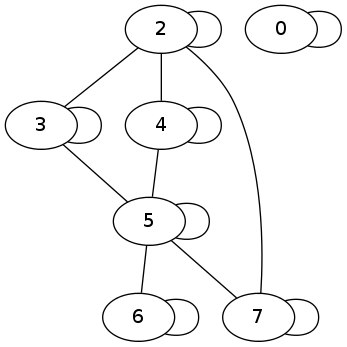
\includegraphics[width=0.3\textwidth]{img/graph1}    
  \structure{Graphs}: Connected? Directed? Redundant Edges? Negative weights?

  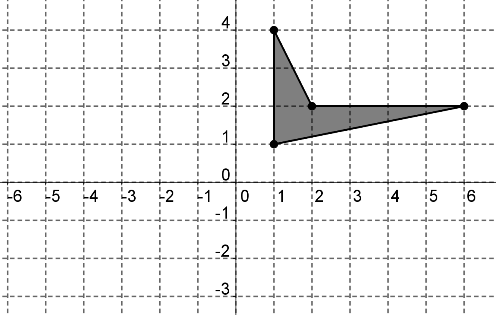
\includegraphics[width=0.3\textwidth]{img/polygon} 
  \structure{Geometry}: Overlapping? Concave? Negative coordinates? Collinear?

  \begin{itemize}
  \item Maximum number of entries;
  \item Zero entries;
  \item ``Wrong'' sort order;
  \item Unsolvable Entries;
  \item Empty sets;
  \item Duplicate items;
  \item Big Numbers ($>$ Long Long);
  \end{itemize}

\end{frame}

\subsection{programming}

\begin{frame}
  \frametitle{NOW you can start to code}
  % TODO: Improve this slide

  You should have done all of the previous steps in writing only!
  Programming distracts from understanding the problem.
  
  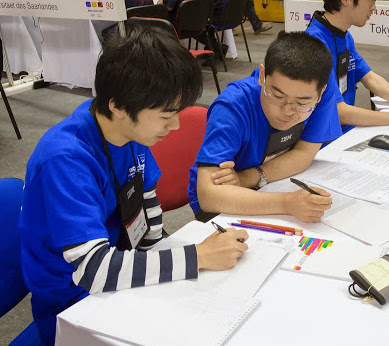
\includegraphics[width=0.6\textwidth]{img/writing}
\end{frame}

\begin{frame}
  \frametitle{Steps for writing the solution}
  \begin{itemize}
    \item Write the input/output first % they are often the same across problems
      % You can't do anything else without I/O
      % Input end condition: EOF, or special cases?
      % Output conditions: precision, newlines, upper/lower case
      
    \item Make the program % Language gimmics: C/C++ pointers, java --
                           % not really designed for programming
                           % contests, you won't be using a lot of
                           % objects - everything is in one file. But
                           % some libraries can be useful. Pascal: WOW-dog
    \item Release often philosophy %TODO:
    \item Testing/Debugging
      % You may be failing on a hard test - write your own secret tests
      % try tests with limit conditions, try tests with random data
      % what are the assumptions of your code? of the problem?
  \end{itemize}
\end{frame}

\begin{frame}
  \frametitle{Speed and Memory Limits}
  Defining speed and memory limits

  Algorithmic efficiency, Memory Efficiency, Programmer efficiency

  % Programming efficiency is useful not only for programming
  % challenges, but also to save you time on more important tasks.

  % Search on 100 elements vs using quicksort for 100 elements
\end{frame}



\subsection{Problem solving example}
\begin{frame}
  \frametitle{Let's apply these steps to a simple problem}
  % Include one error from missing the input
\end{frame}

%%%%%% Week 2 -- Data structures %%%%%%%%%

\section{Data Structures}
\subsection{Introduction}

\begin{frame}
  \begin{center}
    {\bf Data Structures}
  \end{center}
\end{frame}

\begin{frame}
  \frametitle{Data Structures}

  \begin{block}{Data structures are the heart of a program}
    \begin{itemize}
      {\small
      \item Using the correct data type can make a problem much easier;
      \item Using the incorrect data type can make a problem much harder;
      }
    \end{itemize}
  \end{block}

  \begin{block}{The towers of Hanoi}
    \begin{center}
    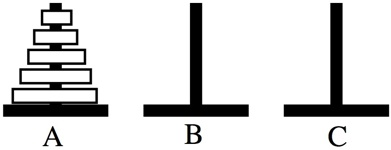
\includegraphics[width=0.5\textwidth]{img/hanoi}
    \end{center}
    \medskip
    QUIZ: How do you represent the data in this problem? 
  \end{block}
\end{frame}

\begin{frame}
  \frametitle{An easy way to visualize the Towers of Hanoi}
  \begin{center}
    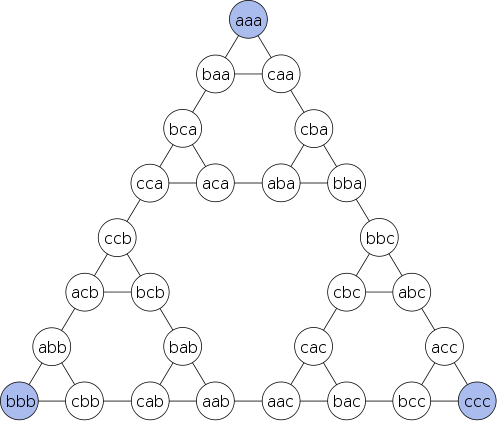
\includegraphics[width=0.7\textwidth]{img/hanoi_graph}
  \end{center}
  {\smaller Image created by nonenmac}
\end{frame}

\begin{frame}
  \frametitle{Explaining the Tower of Hanoi Data Structure}
  \begin{columns}[c]
    \column{0.7\textwidth}
    \begin{itemize}
    \item Each node identifies an state in the problem;
    \item Each character in the string represents one disk and its
      position;
    \item We can have at most 3 state transitions at each state (can
      you prove it?)
    \item To solve the Towers of Hanoi problem, we find the path
      between the start and end states.
    \item (just beware of state explosion)
    \end{itemize}
    \column{0.3\textwidth}    
    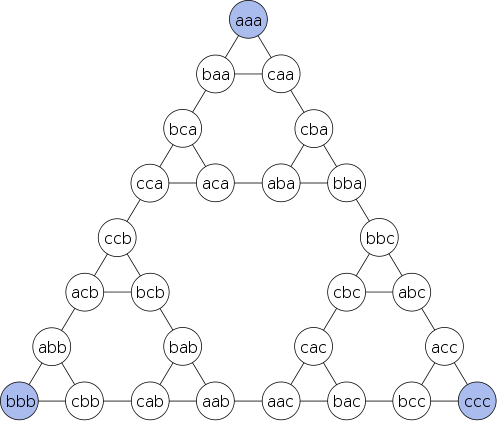
\includegraphics[width=0.9\textwidth]{img/hanoi_graph}
    \vfill
  \end{columns}
\end{frame}

\subsection{Data Structure Library}

\begin{frame}
  \frametitle{Know your data structures!}
  %TODO: Complete this
  %% KNOW your data structures
  % time complexity
  % programming complexity (as we talked before!)
  % common uses
  % common bugs
\end{frame}

\begin{frame}
  \frametitle{Let's talk about libraries}
% It is important then to remember a LIBRARY of interfaces:
% Library: the languages library: How do you use a dictionary in your language of choice?
% Library: your programming portfolio: How many data structures can you remember when you are 
%          thinking about a program? A physical library can be very useful
\end{frame}

%%% Low level data structures
% Array
% Linked List

%%% Medium level data structures
% Stack
% Queue

%%% High level data structures
% Sets, Dictionaries, Priority queues (Dictionary where the keys are orderable)
% Definitions and limitations for each
% Uses and interfaces
% How would you implement them? 

%% Other data structures
% Trees, Graphs, we will talk about these later

%% String
% Strings: computers don't know anything about letters
% String representation: Index x Glyphs
% Encoding: transformation from encoding to glyph.
% Example: ASCII encoding - allows characters to be stored as numbers or as chars
% Why when you write ls -l, the numbers and symbols are first?
% As encoders get bigger and not unified, this starts to get hard


% String structures x string operators (concatenate, set, change order, search -- next week)

%%%%%%%%%%%%%%%%%%

\section{Closing Points}
\subsection{Closing Points}
\begin{frame}
  \frametitle{This week's problems}
  \begin{block}{List of Problems}
    \begin{itemize}
    \item The 3n+1 Problem
    \item Check the Check
    \item Erdos Numbers
    \item Contest Scoreboard
    \end{itemize}
  \end{block}
  \medskip
  Let's give a quick look on each problem
\end{frame}

\begin{frame}
  \frametitle{For the rest of the week:}
  \begin{itemize}
  \item Next class: Bring your solutions and questions!
    \vfill
  \item Submission deadline is 04-19 23:59:59 (Sunday)
    \vfill
  \item Have a nice week!
  \end{itemize}
\end{frame}


% TODO: Complete Friday Class (by friday)
\section{Friday}
\subsection{Friday Class}
\begin{frame}
  \begin{center}
  {\bf Welcome to Friday Class!}
  \end{center}
\end{frame}

\begin{frame}
  \frametitle{Current Solving Stats}
  \begin{itemize}
  \item The 3n+1 Problem -- Solved:
  \item Check the Check -- Solved:
  \item Erdos Numbers -- Solved:
  \item Contest Scoreboard -- Solved:
  \end{itemize}
\end{frame}

\begin{frame}
  \frametitle{Question and hint time!}
  \begin{itemize}
  \item<1> The 3n+1 Problem
  \item<2> Check the Check
  \item<3> Erdos Numbers
  \item<4> Contest Scoreboard
  \end{itemize}
\end{frame}

\begin{frame}
  \frametitle{Let's solve some different problems}
  % TODO: Problem description
  % TODO: Give students 10 minutes to solve the problem
  % TODO: STEP 1 - understanding the problem
  % TODO: STEP 2 - Input/Output, stop conditions
  % TODO: STEP 3 - Problem calculation
  % TODO: STEP 4 - Testing
  % TODO: STEP 5 - Submission

  % TODO: Problem 2
\end{frame}

\end{document}
